\iffalse
\documentclass[10pt,a4paper]{report}
\usepackage[latin1]{inputenc}
\usepackage{amsmath}
\usepackage{amsfonts}
\usepackage{amssymb}
\usepackage{graphicx}
\usepackage{hyperref}
\usepackage{multicol}
\usepackage[margin=0.5in]{geometry}
\usepackage{tikz}
\usepackage[document]{ragged2e}
\usepackage{romannum}
\usetikzlibrary{arrows,shapes.gates.logic.US,shapes.gates.logic.IEC,calc}
\usepackage{titlesec}
\titlespacing{\subsection}{1pt}{\parskip}{3pt}
\titlespacing{\subsubsection}{0pt}{\parskip}{-\parskip}
\titlespacing{\paragraph}{0pt}{\parskip}{\parskip}
\newcommand{\myvec}[1]{\ensuremath{\begin{pmatrix}#1\end{pmatrix}}}
\let\vec\mathbf

\newcommand{\mydet}[1]{\ensuremath{\begin{vmatrix}#1\end{vmatrix}}}
\providecommand{\brak}[1]{\ensuremath{\left(#1\right)}}
\providecommand{\lbrak}[1]{\ensuremath{\left(#1\right.}}
\providecommand{\rbrak}[1]{\ensuremath{\left.#1\right)}}
\providecommand{\sbrak}[1]{\ensuremath{{}\left[#1\right]}}

\begin{document}

\begin{multicols}{2}
\raggedright {
\includegraphics[scale=0.06]{IITH logo.jpg}} \vspace{3mm}\\ \raggedleft Name:SHAIK KHAJA MASTAN AHMED\vspace{2mm}\\ 
\raggedleft Roll No.: FWC22052\vspace{2mm}\\ 
\raggedleft 19pa1a04e9@vishnu.edu.in \vspace{2mm}\\ 
\raggedleft Oct 2022 \vspace{5mm}\\
\end{multicols}

\centering \Large \textbf{MATRIX : CONIC ASSIGNMENT} \normalsize \vspace{10mm}

\begin{multicols}{2}

\section{Problem:}  
\fi
Find the area bounded by the curve $x^2=4y$ and the line $x=4y-2$.
\\
\solution 
	\begin{figure}[!h]
		\centering
 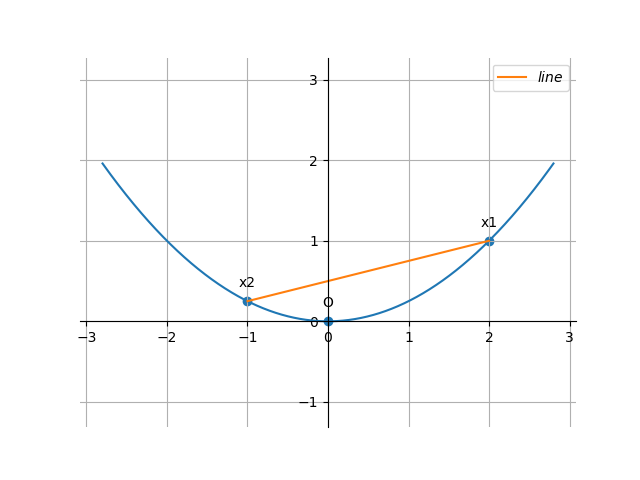
\includegraphics[width=\columnwidth]{chapters/12/8/1/10/figs/conic.png}
		\caption{}
		\label{fig:12/8/1/10}
  	\end{figure}
\iffalse

\section{Solution: }
\raggedright \textbf{Input Parameters :}\\ \vspace{2mm}
\centering Curve Equation : $x^2=4y$. \\ \vspace{1mm}
Line Equation : $x=4y-2$.\\
\vspace{3mm}

\raggedright \textbf{To Find :}\\ \vspace{2mm}
\begin{enumerate}
\item Comparing the given curve equation with the standard equation of the conics and finding it's parameters.
\item Finding the required parameters for the line equation.
\item Finding the Point of Intersection of the to the curve.
\item Finding the area bounded by the curve and the line.
\end{enumerate}

\raggedright \textbf{Step - 1 :}\\ \vspace{2mm}
Curve Equation : $x^2=4y$. \\ \vspace{1mm}
The standard equation of the conics is given as :
\begin{align}
\vec{x}^{\top}\vec{V}\vec{x}+2\vec{u}^{\top}\vec{x}+f=0
\end{align}
\fi
The given curve  can be expressed as a conic with parameters
\begin{align}
	\vec{V} &= \myvec{1 & 0\\0 & 0}, \vec{u} = \myvec{0 \\-2}, f = 0
	\end{align}
\iffalse

\raggedright \textbf{Step - 2 :}\\ \vspace{2mm}
Line Equation : $x=4y-2$. \\ \vspace{1mm}
\fi
The parameters of the given line are
\begin{align}
\vec{q} = \myvec{-2 \\0} , \vec{m}=\myvec{4\\1}
\end{align}
The points of intersection can then be obtained from \eqref{eq:tangent_roots} as
\iffalse

\raggedright \textbf{Step - 3 :}\\ \vspace{2mm}
The points of intersection of the line, \\ 
\begin{align}
L: \quad \vec{x} = \vec{q} + \mu \vec{m} \quad \mu \in \mathbb{R}
\end{align}
with the conic section, \\ 
\begin{align}
	\vec{x}^{\top}\vec{V}\vec{x} + 2\vec{u}^{\top} \vec{x} + f = 0
\end{align}
are given by \\
\begin{align}
\vec{x}_i = \vec{q} + \mu_i \vec{m}
\end{align}
where, \\
{\tiny
\begin{multline}
\mu_i = \frac{1}
{
\vec{m}^T\vec{V}\vec{m}
}
\lbrak{-\vec{m}^T\brak{\vec{V}\vec{q}+\vec{u}}}
\\
\pm
\rbrak{\sqrt{
\sbrak{
\vec{m}^T\brak{\vec{V}\vec{q}+\vec{u}}
}^2
-
\brak
{
\vec{q}^T\vec{V}\vec{q} + 2\vec{u}^T\vec{q} +f
}
\brak{\vec{m}^T\vec{V}\vec{m}}
}
}
\end{multline}
}
\raggedright On substituting $\vec{V},\vec{q} ,\vec{m}$ in the above equation,
we get the values of $\mu$. By substituting the values of $\mu$ in eq(6), \\we get the points of intersection of line with the given curve. \\
\centering $i.e., \vec{x}_1,\vec{x}_2$\\ 
\fi

\begin{align}
\therefore \vec{x}_1=\myvec{2\\1} , \vec{x}_2=\myvec{-1\\ \frac{1}{4}}
\end{align}
\iffalse

\raggedright \textbf{Step - 4 :}\\ \vspace{2mm}
The area bounded by the curve $x^2=4y$ and line $x=4y-2$ is given by\\
\fi
The desired area is then obtained as
\begin{align}
	A&=\int_{x_2}^{x_1} [f(x)-g(x)] \,dx
	\\
	&=\int_{-1}^{2} \brak{\frac{x+2}{4}-\frac{x^2}{4}} \,dx
	\\
	& = \frac{9}{8} 
\end{align}
\iffalse

\raggedright \textbf{Code Link :}\\ \vspace{2mm}
The below link realises the code of the above construction.\\
\begin{center}
\fbox{\parbox{8.5cm}{\url{https://github.com/19pa1a04e9/FWC-IITH/tree/main/Assignment-1/MATRICES/Conic/codes/conic.py}}}
\end{center}


\section{Termux Commands :}
\centering bash rncom.sh ..... Using Shell commands.


\section{Plot :} 
\begin{center}
  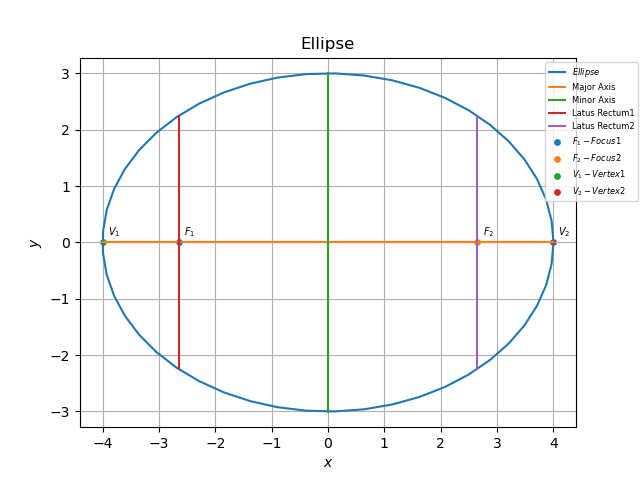
\includegraphics[scale=0.55]{conic.png}
  Figure 1
  	\end{center}

 
\end{multicols}
\end{document}
\fi
